\section{Pre-registration and deviations}
\label{app:deviations}
The analysis plan (\texttt{PREREG.md}) was committed and tagged before any new-corpus statistic was computed. The HateXplain single-corpus results predate it and are replications. The judge addendum (\texttt{PREREG\_ADDENDUM.md}), fixing models, prompts, samples, the parser and the metrics, was committed before any model call; alt-test parameters were added before any alt-test result existed. Table~\ref{tab:dev} lists every departure; the repository's \texttt{DEVIATIONS.md} gives dates and whether results had been seen.

\begin{table*}[t]
\centering\small
\begin{tabular}{@{}p{0.2\textwidth}p{0.5\textwidth}p{0.22\textwidth}@{}}
\toprule
Change & What and why & Results seen before? \\
\midrule
Leave-one-out ceiling & Added a lower end to the ceiling bracket because the mean modal share includes the scored vote. & Only the already-published HateXplain value. \\
Separate seed & New analyses use a new master seed so the earlier HateXplain files still reproduce. & No. \\
Margin definition & Report exactly-one-vote lead and no-plurality separately. & HateXplain only. \\
Hard-item scenario (pre-registered model extended) & Added a second generative model with hard items; extended the gap grid to include negative gaps so false claims exist. & No. \\
Matched-threshold baseline & Compare gates with $z$-tests at matched false-claim rates. & Yes: aggregate gate rates. \\
Gate~v2 and two post-hoc scenarios & Designed after seeing that the $\alpha$ floor loses power; scenarios with the gap on clear items were added because the pre-registered scenario produced no extra false claims. & Yes. \\
Wider $z$ grid & Needed to reach gate~v1's false-claim rate in one scenario. & Yes. \\
Full-data bootstrap & Replaced the subsample bootstrap, whose interval excluded its own point estimate on one emotion. & Yes: first-run intervals. \\
Real-rater study details & Pool/reference split, system models and budgets fixed; one system model re-specified after an infeasibility crash, before any output. & No. \\
Judge pilot & DICES pilot items from DICES-990; a first-word parse rule added after pilot outputs began with a label and then explained. & Pilot only. \\
Sonnet sampling & Claude Sonnet~5.5 rejects temperature~0; default sampling used. & No. \\
\bottomrule
\end{tabular}
\caption{Departures from the pre-registered plan.}
\label{tab:dev}
\end{table*}

\section{All agreement statistics}
\label{app:cross}
\begin{table*}[t]
\centering\small
\begin{tabular}{@{}llrlrrlr@{}}
\toprule
Corpus & Label & $\alpha$ & 95\% CI & AC1 & Raw & Ceiling & $\alpha_{\text{all}}$ \\
\midrule
HateXplain & three way & 0.460 & [0.452, 0.467] & 0.469 & 0.644 & 0.644--0.814 & 0.460 \\
HateXplain & binary & 0.561 & [0.552, 0.571] & 0.592 & 0.789 & 0.789--0.894 & 0.561 \\
MHS & three way & 0.363 & [0.356, 0.370] & 0.585 & 0.686 & 0.695--0.835 & 0.470 \\
MHS & binary & 0.425 & [0.416, 0.434] & 0.634 & 0.775 & 0.781--0.883 & 0.537 \\
Wikipedia Talk & toxicity binary & 0.464 & [0.460, 0.469] & 0.823 & 0.867 & 0.895--0.924 & 0.466 \\
Wikipedia Talk & toxicity score & 0.296 & [0.293, 0.299] & -- & 0.482 & -- & 0.297 \\
DICES-350 & three way & 0.149 & [0.108, 0.190] & 0.400 & 0.556 & 0.613--0.729 & 0.161 \\
DICES-350 & binary & 0.158 & [0.113, 0.208] & 0.317 & 0.623 & 0.661--0.774 & 0.180 \\
DICES-990 & three way & 0.146 & [0.122, 0.172] & 0.482 & 0.602 & 0.659--0.759 & 0.143 \\
DICES-990 & binary & 0.154 & [0.124, 0.183] & 0.449 & 0.666 & 0.706--0.801 & 0.154 \\
\bottomrule
\end{tabular}

\caption{Agreement per corpus and label. Ceiling: leave-one-out to in-sample bracket. $\alpha_{\text{all}}$: all ratings kept instead of at most five per item.}
\end{table*}

\section{Threshold sweep}
\label{app:sweep}
\begin{figure}[h]
\centering
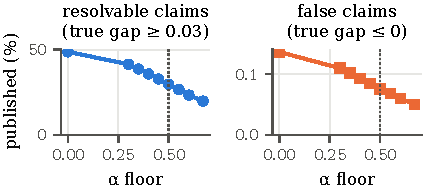
\includegraphics[width=\columnwidth]{figures/alpha_floor_sweep.pdf}
\caption{Gate~v1 under independent rater noise as its $\alpha$ floor varies (dotted: default).}
\end{figure}

\section{HateXplain gaps}
\label{app:retro}
For a paired comparison on $n$ items with discordance $p$ (the share of items exactly one system gets right), a gap $g$ has $z=g/\sqrt{(p-g^2)/n}$, so it is significant at threshold $z^\ast$ only if $p<p_{\max}=g^2(1+n/z^{\ast2})$. Since $p\geq g$, a $p_{\max}$ near $g$ means the gap cannot be resolved by any realistic pair of systems. Values are capped at 100\%.
\begin{table}[h]
\centering\small
\resizebox{\columnwidth}{!}{\begin{tabular}{@{}lrrr@{}}
\toprule
Comparison & Gap & $p_{\max}$ (\%), $z{=}1.96$ & $z{=}2.58$ \\
\midrule
BERT-HateXplain $>$ BiRNN & 0.103 & 100.0 & 100.0 \\
BERT $>$ BiRNN & 0.095 & 100.0 & 100.0 \\
BERT-HateXplain $>$ BiRNN-Attn & 0.077 & 100.0 & 100.0 \\
BERT-HateXplain $>$ CNN-GRU & 0.071 & 100.0 & 100.0 \\
BERT $>$ BiRNN-Attn & 0.069 & 100.0 & 100.0 \\
BERT-HateXplain $>$ BiRNN-HateXplain & 0.069 & 100.0 & 100.0 \\
BERT $>$ CNN-GRU & 0.063 & 100.0 & 100.0 \\
BERT $>$ BiRNN-HateXplain & 0.061 & 100.0 & 100.0 \\
BiRNN-HateXplain $>$ BiRNN & 0.034 & 58.0 & 33.5 \\
CNN-GRU $>$ BiRNN & 0.032 & 51.4 & 29.7 \\
BiRNN-Attn $>$ BiRNN & 0.026 & 33.9 & 19.6 \\
BiRNN-HateXplain $>$ BiRNN-Attn & 0.008 & 3.2 & 1.9 \\
BERT-HateXplain $>$ BERT & 0.008 & 3.2 & 1.9 \\
CNN-GRU $>$ BiRNN-Attn & 0.006 & 1.8 & 1.0 \\
BiRNN-HateXplain $>$ CNN-GRU & 0.002 & 0.2 & 0.1 \\
\bottomrule
\end{tabular}
}
\caption{Published HateXplain test-accuracy gaps and the largest disagreement rate at which each is resolvable.}
\end{table}

\section{Judge experiment details}
\label{app:judges}
\paragraph{Models.} Claude Haiku~4.5 (\texttt{claude-haiku-4-5-20251001}, temperature 0, 16 output tokens) and Claude Sonnet~5.5 (\texttt{claude-sonnet-5-5}, thinking off, effort low, 64 output tokens, default sampling because the model rejects temperature 0) through the Anthropic Message Batches API; GPT-4.1-mini (snapshot \texttt{gpt-4.1-mini-2025-04-14}, temperature 0, seed 0, 16 output tokens) through the OpenAI Chat Completions API; Qwen2.5 14B (\texttt{qwen2.5:14b}) and gpt-oss 20B (\texttt{gpt-oss:20b}, reasoning effort low) through Ollama on one Apple M4 Max, temperature 0, seed 0. No server-side fallback to another model was enabled. We excluded a free API tier whose terms state that submitted content is used to improve the provider's products, and a free tier whose daily token limit would have required more than a week.

\paragraph{Prompts.} One system prompt per corpus (the repository's \texttt{prompts/}, hashed in \texttt{PREREG\_ADDENDUM.md}), paraphrasing the corpus's question: HateXplain (hatespeech / offensive / normal), MHS (``Is this comment hate speech?'' yes / unclear / no), Wikipedia Talk (five-point toxicity scale, binarised at toxic), DICES (is the chatbot's final response unsafe: yes / no / unsure). The item text is the user message; there are no examples.

\paragraph{Sample and scoring.} Items with at least three ratings in the capped matrix; a seeded sample of 1,000 per corpus (all 350 for DICES-350); one seeded held-out rater per item. Outputs are parsed strictly (the answer is a label), then by first word, then leniently (exactly one label word); anything else is unusable. A formatting pilot on five items per corpus outside the sample led to the first-word rule; no evaluation output was seen before it was fixed.

\paragraph{Alternative Annotator Test.} Implemented from \citet{calderon2025alternative}: per annotator $j$, alignment $S(\cdot,x_i,j)$ is the mean agreement with the item's other annotators; win indicators $W^f=\mathbb{1}\{S_f\geq S_h\}$ and $W^h=\mathbb{1}\{S_h\geq S_f\}$; a one-sided $t$-test of $H_0{:}\ \rho^f_j\leq\rho^h_j-\varepsilon$ on $d=W^h-W^f$; Benjamini--Yekutieli across annotators; pass if the winning rate is at least 0.5. For DICES we use all ratings (123 raters per item), because the five-rating cap leaves no DICES rater with 30 items. We do not use the paper's skew correction.

\paragraph{Cost.} The three API judges used \$\jCostUsd at list prices (Batch API rates for Anthropic). Token counts per judge and corpus are in \texttt{results/judge/analysis.json}.

